

\begin{figure}[t]
\begin{center}
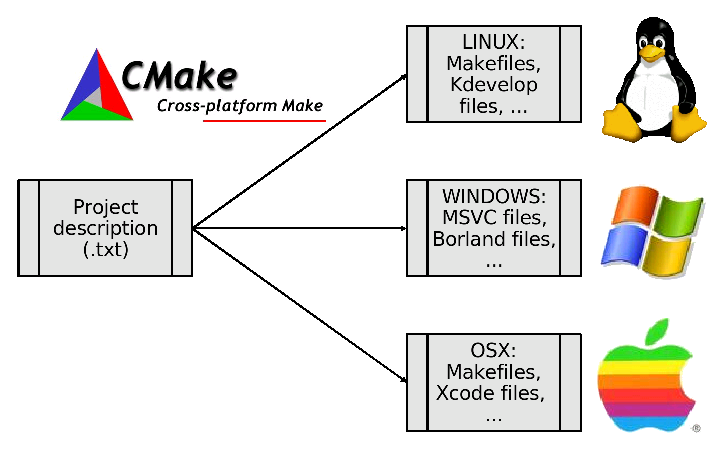
\includegraphics[height=3.5cm]{fig-cmake}
\ \ \ \ \ \ 
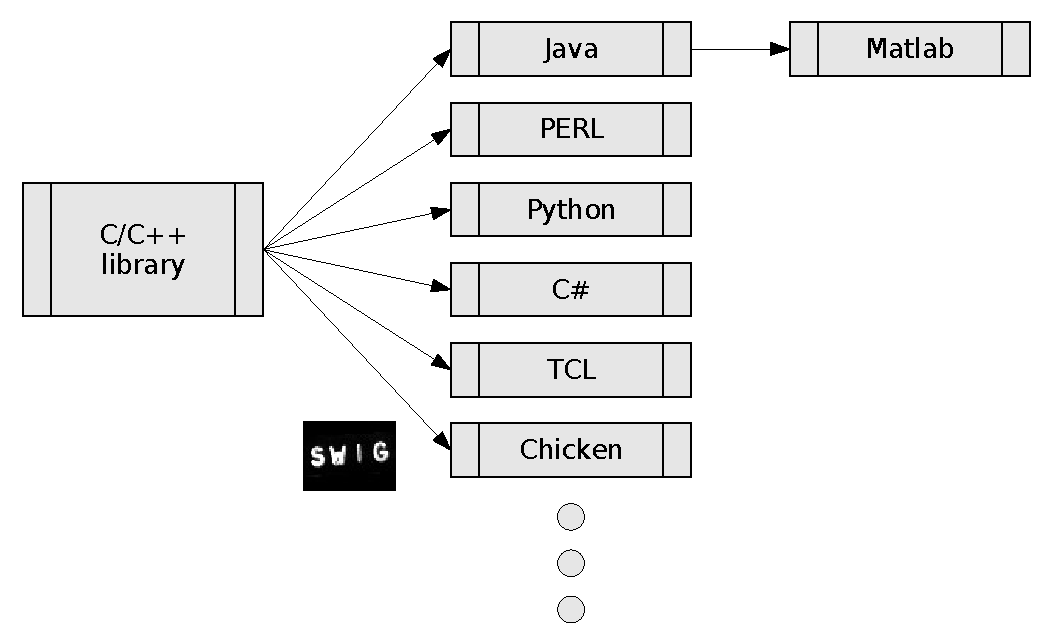
\includegraphics[height=3.5cm]{fig-swig}
\caption{
%
\label{fig:build}
%
With the aid of a set of free and open source tools, 
a C/C++ based project like YARP can have a very
wide reach.
%
C/C++ source code is quite portable and widely supported, but the
infrastructure needed to compile such programs varies a great 
deal.  Tools like autoconf and automake have smoothed over
the differences for UNIX-like systems. CMake (left) goes
further and makes projects easy to compile within a
wide range of integrated development environments
(including UNIX-like systems, but also Microsoft Visual C++,
Apple Xcode, Kdevelop, etc).
%
For operating-system dependent functions, we use the free
and open source ACE library.
%
SWIG (right) takes C/C++ source code and generates ``wrappers''
for it, usable from many different languages (including Matlab
via Java).
%
%
}
\end{center}
\end{figure}


\section{A software ecology}


%Software development for humanoid robots is somewhat of a back-water.
%Although it is a topic that excites the public imagination, the
%actual resources devoted worldwide are quite low.  The Japanese
%government and car manufacturers have invested in some high-profile
%projects...


Many robot projects are ``black holes'', in terms of software.  A lot
of software gets sucked in, but very little comes out.  Once a piece
of software has been adapted to a particular robot, it takes a lot
of work to extricate it again and apply it to another.
%
Obviously the answer to this problem is modularity.  So there are 
now many architectures/frameworks/... for modular robot systems.
The prime concern for any such system should be that it is not
a ``black hole'' -- that once a piece of software has been adapted
to a particular framework, it takes a lot of work to extricate it
again and apply it to another.  That would be a bit self-defeating.

So modularity alone is not a solution to software reuse, since 
different organizing frameworks or architectures may be mutually
incompatible.  It is import that modules developed can fit
into a broader ``ecology'' than just the framework/architecture
of the developers.  By ecology, we mean the messy complicated
collection of niches world-wide in which software development occurs.

%We study YARP from this perspective.  How sticky is resultant user
%code to the robot and to the framework itself?





\subsection{C/C++}

We decided to use C++ as the main language for development. This 
is motivated by the fact that C++ is an object oriented language
that is widely used by many developers in the world, and is well 
supported and portable on almost all the available platforms. 
Perhaps more importantly for robotics, C++ allows writing very 
efficient code and interfacing with the hardware at the lowest 
level.

The drawback is that the compile process varies a lot depending 
on the platform and development environment. For example Linux 
and Cygwin developers use mostly Makefiles, whereas Microsoft Windows 
developers may prefer Visual Studio project files. 
Altough C++ has reached a fairly good level 
of portability which allows, with a reasonable effort, writing 
applications that compile on all platforms, it is still very 
common to have to wrestle to port code that was written for 
a platform to another. On the other hand, following a 
modular approach, we would like our software to be as flexible 
as possible and adapt to needs of the user and the platform that 
he uses. In YARP, when possible, unavoidable dependencies 
have been made as localized as possible to modules that can be 
compiled or not depending on the underlying system and user 
choices. So for example applications that require a GUI gets 
compiled only when the supporting libraries (mainly GTK+) 
is installed in the system. Another example is the mathematical
library which is built on top of the GNU Scientific Library. 
The idea is that only the modules that only and \emph{all} the 
modules that can be compiled are actually built.

To avoid asking the user to go through a tedious and long process 
of manual configuration, a program automatically inspects the 
system and generates the files necessary to compile YARP 
on the host system (e.g. make files in Linux systems, or Visual 
Studio project files in Windows). This simplifies development, 
because it is no longer required to distribute build files 
for all possible platforms.

Among the available tools for automatic configuraton of 
software packages, we decided to use CMake
(see Figure~\ref{fig:build}). CMake is 
cross-platform open-source, make system. It produces 
build files for the environment of choice (e.g. makefiles
for Unix, Borland and MinGW and project files for all 
Microsoft compilers) starting from a language independent 
description. The language of CMake is powerful enough
to support a flexible configuration process based 
on the packages that are available in the system and 
the preferences of the user. Through 
CMake the build process of YARP is robust, simple and 
flexible.
%
%Has the excellent property of being simpler than making Makefiles
%or configuring a project, when external libraries are involved.
%
%The big downside is that the language is unfamiliar and a bit ugly.
%It is simple and well-documented, but quirky.  An alternative with
%some similar properties, scons, uses python instead.  The ant system
%uses with java also seems cleaner.  However, it gets the job
%done, and has the huge advantage of not being dependent on an
%external language being installed.
%
CMake is free and open-source, with a healthy community of 
developers.



%%\subsection{Repositories}
%%sourceforge.  debian.


\begin{figure}[t]
\begin{center}
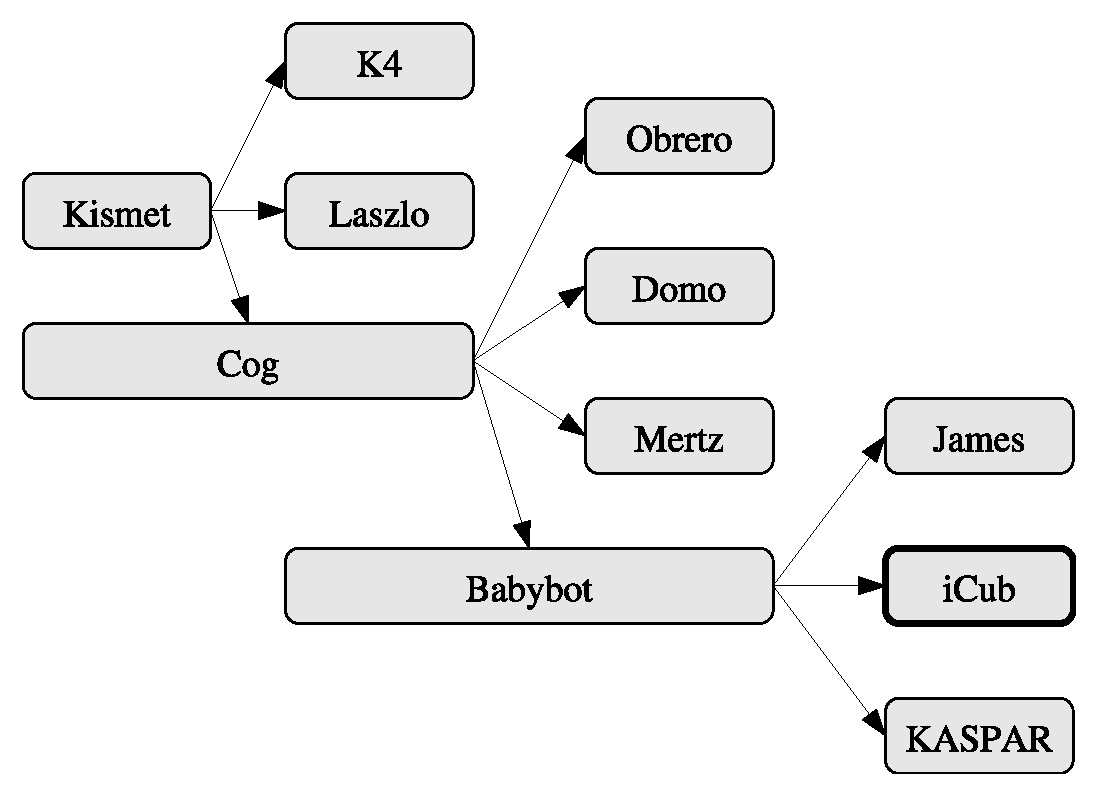
\includegraphics[height=5cm]{fig-family}
\caption{
%
\label{fig:family}
%
A potted history of YARP.  YARP was born on Kismet (CITE),
grew up on Cog and BabyBot (CITE), and serves as the
software architecture for the iCub humanoid (CITE).
%
Along the way other humanoids have also used the system.
%
With iCub, we are trying to create some hardware ``genes''
that can travel along too, so each robot does not need to
be designed from scratch.
%
%
}
\end{center}
\end{figure}



\subsection{Free Software}

The ability to integrate software modules into a system
depends not just on the technical constraints attached
to their use, but also the cultural constraints
(be they social, legal, or commercial) they carry.
%
For example, whether two modules can be integrated
can depend not just on their interfaces but also on
the conditions under which use of the modules
is permitted by their respective creators,
and what conditions the integrator wishes to 
apply to the aggregated system.  
%
This adds a great deal of complexity to the process
of integration.
%
In general, software produced under conditions where the 
creator has strong opinions about how it should be 
used, and enforces those opinions in licensing
and other measures, does not make a good module 
to build on.
%
It is possible, but painful.

The Free Software model is an alternative that strikes a different
balance between creator and integrator.  It proposes a set of standard
freedoms which should be granted with software. Taken together make
the software actually useful as building blocks without excessive
social/legal/commercial complexity.  The freedoms are enforced using
copyright law principles that apply to most of the world.

The Free Software model says nothing about the cost of software,
although it does tend to contribute to commoditization, driving the
cost of ``infrastructure''-like software such as webservers and
operating systems down.  Free software should not be confused with
``freeware''.  Freeware software is available without charge but may
have complex social/legal/commercial terms attached, and may
or may not grant the freedoms associated with free software
(usually not).

The effectiveness of free and open software is 
becoming better understood from a business
perspective \cite{vonkrogh2006promise}.
%
The free and open model has had a crucial 
effect in the field of embedded devices,
a large and growing market that overlaps
with robotics, spurred by the existence
of embedded Linux \cite{henkel2006selective}.



%% Has the revolutionary benefit that the user is not trapped in the role
%% of being a ``consumer'' of software, but can also be a publisher of
%% the changes, additions, and integrative work they do in an effective
%% form.  This is achieved by explicitly granting far more rights to
%% users than they have under the law of most countries, contrasting with
%% agreeably with the formerly more common practice of attempting to
%% minimize user rights.  These rights are typically granted
%% conditionally; a user may only make use of these extended rights if
%% (for example) distributed code is always available in its most useful
%% original (source) form, with compatible freedoms attached to it.  This
%% condition seeks to balance freedoms of individuals versus benefit to
%% the group.  The existence of code in usable form with freedoms 
%% attached can benefit many people;

%%The freedom to distribute code in obscure (compiled) forms



%%Split between people who emphasize pragmatic concerns and those
%%who emphasize freedom.  Just cite the issue, no need to revisit
%%it here.





\subsection{Interoperating with other architectures/frameworks}

The closest project in spirit to YARP is that of the Player project
\cite{vaughan2006reusable}.  The Player/Stage software collection is 
widely used in the field of mobile robotics, and is the nucleus of
a healthy, pragmatic community of developers.  
%
Rudimentary interoperability is possible between these projects.
Player contains a ``yarpimage'' driver which can accept images
from a YARP Network.  A ``stage'' driver has been developed
for YARP, which gives access to the 2D srobot simulator of that
name from a YARP Network.
%
The driver mechanism in both projects gives a very straightforward way
to integrate quickly with what would otherwise be incompatible
middleware.

Both projects are free and open source.  They both have documented
network protocols.  Both have made an effort to allow different
transports, and to be portable.  Given all these similarities,
it is reasonable to wonder whether the projects could be merged.
%
From the YARP perspective, there doesn't seem any compelling reason to
do so right now; individuals who've needed parts of both systems have
been able to do so through the driver mechanisms.
%
From the Player perspective, YARP's dependence on ACE is probably
undesirable, and YARP uses more C++ features than the C-with-Classes
style of Player (which is probably a better idea for portability).
Also, we use different build machinery (autotools versus CMake).
%
Due to recent changes in Player, communications could probably be
adapted.  Devices are different in YARP and Player.  YARP starts
with just a thin C++ wrapper which permits direct function calls;
Player devices require message passing (even if the message passing
is just internal rather than across a network).


%%serialization / message passing

%%Player's communication model,
%%which used to be client/server, has recently been expanded to
%%be more flexible, and seems to be getting closer to a peer-to-peer
%%mechanism such as YARP.



%%Categories from \cite{collett2005player}:


